\documentclass[a4paper, 14pt]{extarticle}

\usepackage{../../latexDependencies/misc/preamble2}

\geometry{a4paper}

% Название дисциплины
\newcommand{\subject}{Теория вероятности и математическая статистика} 

% Тип работы
% lab - для лабораторной работы 
% hw  - для домашней     работы
\newcommand{\task}{lab} 

% Номер работы
\newcommand{\taskNumber}{3} 

% Название работы
\newcommand{\taskNameOne}{Моделирование выборки из абсолютно непрерывного } 
\newcommand{\taskNameTwo}{закона распределения методом обратных функций.} 

% Имя студента
\newcommand{\studentName}{Очкин Н.В.}

% Имя преподававателя
\newcommand{\teacherName}{Облакова Т.В.}

% Группа
\newcommand{\group}{ФН11-52Б}

% Вариант
\newcommand{\variant}{9}

\begin{document}

\graphicspath{ {../../latexDependencies/images} } 
\normalsize

\newcommand{\printTask}{%
    \ifthenelse{\equal{\task}{lab}}{%
        лабораторной%
    }{%
        \ifthenelse{\equal{\task}{hw}}{%
            домашней%
        }{%
            Неизвестный тип задания%
        }%
    }%
}

\begin{titlepage}

    \begin{center}
        {\footnotesize \itshape Федеральное государственное бюджетное 
                       образовательное учреждение высшего образования}
    \end{center}

    \begin{minipage}[c]{0.1\textwidth}
        
\includegraphics[width=1.1\textwidth]{iconBMSTU}
    \end{minipage}
    \hfill
    \begin{minipage}[c]{0.9\textwidth}
        \centering
        \itshape
        \bfseries
        \small
        \guillemotleft Московский государственный технический университет \\
        имени Н.Э. Баумана\guillemotright \\
        (национальный исследовательский университет) \\
        (МГТУ им. Н.Э. Баумана) 
    \end{minipage}

    \vspace{0.5cm}
    \noindent\rule{\textwidth}{2pt} \\

    \noindent\uline{\textbf{ФАКУЛЬТЕТ} ФУНДАМЕНТАЛЬНЫЕ НАУКИ} \\
    \vspace{-5pt} \\
    \noindent\uline{\textbf{КАФЕДРА} ВЫЧИСЛИТЕЛЬНАЯ МАТЕМАТИКА И МАТЕМАТИЧЕСКАЯ} \\
    \vspace{-5pt} \\
    \noindent\uline{ФИЗИКА (ФН11)} \\
    \vspace{-5pt} \\
    \noindent\uline{\textbf{НАПРАВЛЕНИЕ ПОДГОТОВКИ} МАТЕМАТИКА И КОМПЬЮТЕРНЫЕ} \\
    \vspace{-5pt} \\
    \noindent\uline{НАУКИ (02.03.01)} \\

    \begin{center}
        \bfseries
        \textsc{О т ч е т} \\[10pt]
        по \printTask {} работе \textnumero {} \taskNumber
    \end{center}

    \vspace{10pt}

    \hspace{10pt} 
    \noindent \textbf{Название \printTask {} работы:} \par
    \vspace{5pt}
    \hspace{10pt} 
    \noindent \textbf{\uline{\taskNameOne}} \vspace{5pt} \\
    \null\hspace{31pt} 
    \textbf{\uline{\taskNameTwo}} \vspace{5pt} 

    \vspace{10pt}

    \begin{center}
        \bfseries
        Вариант \textnumero {} \variant
    \end{center}

    \vspace{20pt}

    \hspace{10pt} 
    \noindent \textbf{Дисциплина:} \par
    \vspace{10pt}
    \hspace{10pt} 
    \noindent {\large \subject}

    \vspace{10pt}

    \begin{flushright}
        \renewcommand{\arraystretch}{3}
        \begin{tabular}{r r r}
            \multicolumn{1}{l}{Студент группы \uline{\group}} & 
            $\quad \underset{\text{(Подпись, дата)}}{\underline{\hspace{3cm}}} \quad$ & 
            \multicolumn{1}{c}{$\underset{\text{(И.О. Фамилия)}}{\uline{\textbf{\studentName}}}$} \\

            \multicolumn{1}{l}{Преподаватель} & 
            $\quad \underset{\text{(Подпись, дата)}}{\underline{\hspace{3cm}}} \quad$ & 
            \multicolumn{1}{c}{$\underset{\text{(И.О. Фамилия)}}{\uline{\textbf{\teacherName}}}$} \\
        \end{tabular}
    \end{flushright}

    \vfill

    \begin{center}
        \small
        Москва, 2024
    \end{center}
\end{titlepage}


\newgeometry{left=25mm, right=25mm, top=20mm, bottom=20mm}

\graphicspath{ {../../latexDependencies/images/LW3} }

% Customize section, subsection, subsubsection and paragraph styles
\titleformat{\section}
  {\normalfont\large\bfseries}{\thesection}{1em}{}

\titleformat{\subsection}
  {\normalfont\normalsize\bfseries}{\thesubsection}{1em}{}

\titleformat{\subsubsection}
  {\normalfont\small\bfseries}{\thesubsubsection}{1em}{}

\titleformat{\paragraph}
  {\small\small\bfseries}{\theparagraph}{1em}{}

\thispagestyle{empty}

\null\newpage

\setcounter{tocdepth}{5}
\setcounter{secnumdepth}{5}

\pagenumbering{roman}

\tableofcontents
\newpage

\pagenumbering{arabic}
\setcounter{page}{1}

\setstretch{1}
\linespread{1.1}

\setlength{\parindent}{0pt}

\fontsize{12pt}{16pt}\selectfont

% --------------------------------------START--------------------------------------

\section{Задание}\vspace{-20pt}\rule{\linewidth}{0.1mm}

\begin{enumerate}
  \item Для данного $n$ методом обратных функций смоделируйте выборку 
  из закона распределения с заданной плотностью  $p(x)$.
  \item Для полученной выборки найдите гистограмму относительных частот. 
  Постройте на одном рисунке графики теоретической плотности $p(x)$ и 
  гистограмму относительных частот.
  \item Вычислите выборочное среднее и выборочную дисперсию и сравните с 
  истинными значениями этих характеристик.
  \item Используя неравенство \high{Dvoretzky-Kiefer-Wolfowitz}, 
  постройте 90\% доверительный интервал для функции распределения $F(x)$.
\end{enumerate}

Приведите графическую иллюстрацию

\section{Исходные данные}\vspace{-20pt}\rule{\linewidth}{0.1mm}

\begin{equation*}
  \text{Вариант: }9 \qquad n: 120
\end{equation*}
\begin{equation}
  \scalebox{1.25}{$p(x) = \cfrac{1}{\sqrt{0.4 \pi}x} e^{-(\ln{x} - 2)^2 / 0.4}, \quad x > 0$}
\end{equation}

\section{Решение}

\subsection{Часть 1}\vspace{-20pt}\rule{\linewidth}{0.1mm}
Для данного $n$ методом обратных функций смоделируйте выборку 
из закона распределения с заданной плотностью  $p(x)$.\\

\subsubsection{Функция распределения}\vspace{-20pt}\rule{\linewidth}{0.1mm}

Найдем функцию распределения:
\begin{equation}
    F_X(x) = \int_{-\infty}^{x} f_X(t) dt, \quad \text{где}
\end{equation}
$f_X(x)$ - плотность распределения.\\

Подставим (1) в (2):
\begin{gather*}
    F_X(x) = 
    \int_{0}^{x} \cfrac{1}{\sqrt{0.4 \pi}y} e^{-(\ln{y} - 2)^2 / 0.4} dy = \\[1em]
    = \left[\hspace{5pt}
    \begin{aligned}
        & t          = \frac{\ln(y)-2}{\sqrt{0.4}}          \qquad & dt &   = \frac{1}{y \sqrt{0.4}} dy   \\
        & \ln(y) - 2 = t \sqrt{0.4}                         \qquad & dy &   = y \sqrt{0.4} dt             \\
        & \ln(y)     = t \sqrt{0.4} + 2                     \qquad & x: & \hspace{5pt} t = \frac{\ln(x)-2}{\sqrt{0.4}} \\
        & y          = \exp \left[ t \sqrt{0.4} + 2 \right] \qquad & 0: & \hspace{5pt} t = -\infty                     \\ 
    \end{aligned}\,
    \hspace{5pt}\right] = \\[1em]
    = \cfrac{1}{\sqrt{0.4 \pi}} \int_{-\infty}^{\frac{\ln(x)-2}{\sqrt{0.4}}} e^{\left[ -t \sqrt{0.4} -2 \right]} 
    \cdot e^{-t^2} \cdot e^{\left[ t \sqrt{0.4} +2 \right]} \cdot \sqrt{0.4} dt = \\[1em]
    = \cfrac{1}{\sqrt{\pi}} \int_{-\infty}^{\frac{\ln(x)-2}{\sqrt{0.4}}} e^{-t^2} dt 
    = \frac{1}{\sqrt{\pi}} \left( \int_{-\infty}^{0} e^{-t^2} dt + \int_{0}^{\frac{\ln(x)-2}{\sqrt{0.4}}} e^{-t^2} dt \right) = \\[1em]
    = \frac{1}{\sqrt{\pi}} \left( \frac{\pi}{2} \text{erf} (t) \bigg|^0_{-\infty} + \frac{\sqrt{\pi}}{2} \cdot 
    \text{erf} \left( \cfrac{\ln(x)-2}{\sqrt{0.4}} \right) \right) \oeq
\end{gather*}\\
\vspace{10pt}
\hdashrule[0.5ex][c]{1\textwidth}{0.4pt}{3mm}
\begin{center}
    где erf(x) - \textbf{функция ошибок} (также называемая функция ошибок Гаусса).\\
\end{center}

\begin{minipage}[c]{0.5\textwidth}
    \begin{equation*}
        \scalebox{1.25}{$\text{erf} (x) = \cfrac{2}{\sqrt{\pi}} \int_{0}^{x} e^{-t^2} dt$}
    \end{equation*}
\end{minipage}
\hfill
\begin{minipage}[c]{0.5\textwidth}
    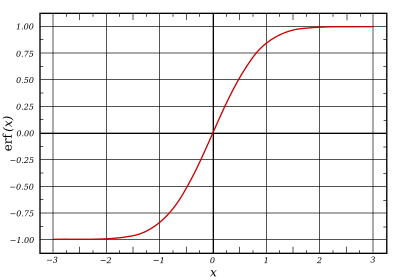
\includegraphics[width=1\textwidth]{Error_Function.svg}
\end{minipage}\\

{\footnotesize \textbf{Примечание:} из графика видно, что erf(0) = 0, erf($-\infty$) = -1}

\hdashrule[0.5ex][c]{1\textwidth}{0.4pt}{3mm}

\begin{gather*}
    \oeq \hspace{3pt} \frac{1}{\pi} \left( \frac{\pi}{2} \left( 0 - \left( -1 \right) \right) + 
    \frac{\pi}{2} \cdot \text{erf} \left( \cfrac{\ln(x)-2}{\sqrt{0.4}} \right) \right) = \\[1em]
    = \frac{1}{\pi} \left( \frac{\pi}{2} + \frac{\pi}{2} \cdot \text{erf} \left( 
    \cfrac{\ln(x) - 2}{\sqrt{0.4}} \right) \right) = \\[1em]
    = \cfrac{1}{2} + \cfrac{1}{2} \text{erf} \left( \cfrac{\ln(x) - 2}{\sqrt{0.4}} \right)
\end{gather*}\\
\vspace{-10pt}
В конечном итоге, функция распределения имеет вид\\[1em]
\begin{equation}
    F_X(x) = \cfrac{1}{2} + \cfrac{1}{2} \text{erf} \left( \cfrac{\ln(x) - 2}{\sqrt{0.4}} \right)
\end{equation}

\subsubsection{Обратная функция}\vspace{-20pt}\rule{\linewidth}{0.1mm}

Так как для нахождения обратной функции распределения требуется найти обратную 
функцию ошибок, что аналитически сделать сложно, воспользуемся численными методами.

\paragraph{Метод Ньютона}\vspace{-20pt}\rule{\linewidth}{0.1mm}

Для нахождения обратной функции воспользуемся методом касательных (Ньютона). \\
Рабочая формула
\begin{equation*}
  x_{n+1} = x_n - \cfrac{f(x_n)}{f'(x_n)}
\end{equation*}
Вообще говоря, метод используется для нахождения корня заданной функции. Так что 
для нахождения обратной функции $y = f(x)$, т.е. $x = f^{-1}(y)$ будем искать 
решение уравнения: $f(x) - y = 0$
\begin{equation}
  x_{n+1} = x_n - \cfrac{f(x_n) - y}{(f(x_n) - y)'_x} = 
  x_n - \cfrac{f(x_n) - y}{f'(x_n)}
\end{equation}
Погрешность $\varepsilon$ возьмем равной 1e-6.

\paragraph{Метод центральных разностей}\vspace{-20pt}\rule{\linewidth}{0.1mm}

Производные будем искать методом центральных разностей.\\
Рабочая формула
\begin{equation}
  f'(x) \approx \cfrac{f(x+h) - f(x-h)}{2h}
\end{equation}
Погрешность определяется как $O(h)$, $h$ примем равной 1e-6.\\

Подставив (5) в (4), получим:
\begin{equation}
  x_{n+1} = x_n - \cfrac{(f(x_n) - y) \cdot 2 h}{f(x_n + h) - f(x_n - h)}
\end{equation}

\subsubsection{Реализация численного нахождения обратной функции}

\paragraph{Реализация метода центральных разностей}\vspace{-20pt}\rule{\linewidth}{0.1mm}



\paragraph{Реализация метода Ньютона}\vspace{-20pt}\rule{\linewidth}{0.1mm}



\end{document}
